\documentclass[a4paper, 11pt, ngerman, fleqn]{article}
\usepackage[utf8]{inputenc}
\usepackage{babel}
\usepackage{ngerman}
\usepackage{coordsys,logsys,color}
\usepackage{german,fancyhdr}
\usepackage{hyperref}
\usepackage{texdraw}				
\usepackage[T1]{fontenc}					
\usepackage{amsmath,amsfonts,amssymb}	
\usepackage[normalem]{ulem}	
\usepackage{listings}
\usepackage{graphicx}


\hypersetup{colorlinks=true, breaklinks=true, linkcolor=darkblue, menucolor=darkblue, urlcolor=darkblue, citecolor=darkblue}

\lhead{\sc{Reviewdokument PECTO}}

\pagestyle{fancy}

\renewcommand{\familydefault}{cmss}

\definecolor{fgcgray}{rgb}{0.4, 0.4, 0.4}
\definecolor{darkblue}{rgb}{0,0,.6}
\definecolor{glossb}{rgb}{0,0,0.38}
\newcommand{\titlefont}[1]{\textcolor{black}{\fontseries{bx}\fontshape{n}\fontsize{30}{0pt} \selectfont #1}}
\newcommand{\titlepagef}[1]{\textcolor{black}{\fontseries{bx}\fontshape{n}\fontsize{14}{0pt} \selectfont #1}}

\newcommand{\gloss}[1]{\textcolor{glossb}{\fontsize{11}{0pt}\selectfont #1}}



\addtolength{\oddsidemargin}{-1.0cm}
\addtolength{\evensidemargin}{-1.0cm}
\addtolength{\headwidth}{2.0cm}
\addtolength{\textwidth}{2.0cm}

\setlength{\parindent}{0cm}

\renewcommand{\labelitemi}{$\circ$}
\renewcommand{\labelitemii}{$\diamond$}

\newcommand{\spaceline}[1][8pt]{\vskip #1}
\newcommand{\attrname}[1]{\textcolor{fgcgray}{\scriptsize #1}}

\newcommand{\comment}[1]{\spaceline[5pt] \textcolor{fgcgray}{\scriptsize #1} \spaceline[15pt]}

\makeatletter

\newcommand*{\project}[1]{\gdef\@project{#1}}

\usepackage[]{siunitx}


\def\@maketitle{
  %\begin{titlepage}
   
  \begin{center}
      \titlepagef{Softwareprojekt 2016}
      \spaceline
  \end{center}
  
  \begin{center}
      \parbox{\textwidth}{
        \spaceline
        \centering{\titlefont{\@title}}
        \par
        \spaceline
      }
  \end{center}
  
  \begin{center}
    \titlepagef{Rapid Layer-2 Encryption Framework}
    \spaceline[2em]
  \end{center}
  
  \begin{center}
  \begin{tabbing}
  Yannic Faulwetter \qquad \=
  Michael Fuchs \qquad \=
  Milan Haverkock \qquad \=
  Felix Seidel \\
  Daniel Scheliga
  \>Tobias Schubert
  \>Jörn Weisensee  
  \>Nils Winkelbach
  \end{tabbing}
  \end{center}
 
  
  \spaceline[3em] {
    \begin{flushright}
    \begin{tabular}[t]{rl}
      \attrname{letzte Änderung:} & \@date
    \end{tabular}
    \end{flushright}
    \par
  }
  \spaceline[5.5em]
  %\end{titlepage}
}

\begin{document}
\title{Reviewdokument: PECTO}
\vspace{3 in}
\maketitle
\clearpage

\section*{Reviewdokument}
Das Reviewdokument ist in zwei Teile aufgeteilt. 
Zum einen enthält es die Ergebnisse der Planung, zum anderen werden hier auch die des Entwurfes festgehalten.
Die Ergebnisse der Planung beinhalten das Vorgehensmodell, Aufwands- und Risikoabschätzung, Meilensteine und diverse organisatorische Vereinbarungen. Im Entwurf werden die Resultate der aktuellen Iteration, Festlegungen für die nächste Iteration und die verwendeten Werkzeuge aufgezeigt.

\section{Ergebnisse der Planung}

Ein großer Teil der Planung eines Projektes spiegelt sich im Pflichtenheft wieder. Dort wird die Anforderungsanalyse festgehalten, Ziele deklariert, sowie Entscheidungen und Produktinformationen niedergeschrieben.

\subsection{Vorgehensmodell}

Diese Modellart ist eine Beschreibung des Vorgehens, welches passend zu den Anforderungen des Projektes gewählt werden sollte. 
Bei der Auswahl und Entscheidung für ein spezielles Vorgehen spielen Anforderungen, Richtlinien und Kenntnisse über den Ablauf eine Rolle.

	\begin{description}
	\leftskip=0,8cm
		\item[Gewähltes Vorgehen:] Nach dem Vorbild von Scrum wurde ein agiles Vorgehen, in insgesamt 3 Sprints aufgeteilt, beschlossen. 
		Jeder Sprint endet mit einem der Vorstellungstermine, die uns durch das Softwareprojekt vorgegeben sind. 
		
		\item[Projektspezifische Anpassungen:] Einzelpersonen haben mehrere Rollen, da der Aufwand für jede Rolle sehr unterschiedlich ist.
	\end{description} 
	
\subsubsection{Vorgehensspezifische Inhalte}
Da für dieses Projekt ein agiles Vorgehen gewählt wurde, mussten hierbei die Meilensteine, welche das Ziel am Ende jeder Iteration sind, definiert werden.
Diese geben einen Ausblick auf den Leistungsumfang des Systems, welchen es bis zum Ende der jeweiligen Iteration abdecken soll.

\subsection{Aufwandsabschätzung}
Mit der Aufwandsabschätzung wird versucht, die verschiedenen Teile des Projektes anhand von Aufwands- und Komplexitätskriterien einzuteilen. (siehe Abbildung 1)
\clearpage
	\begin{figure}
		\begin{center}
			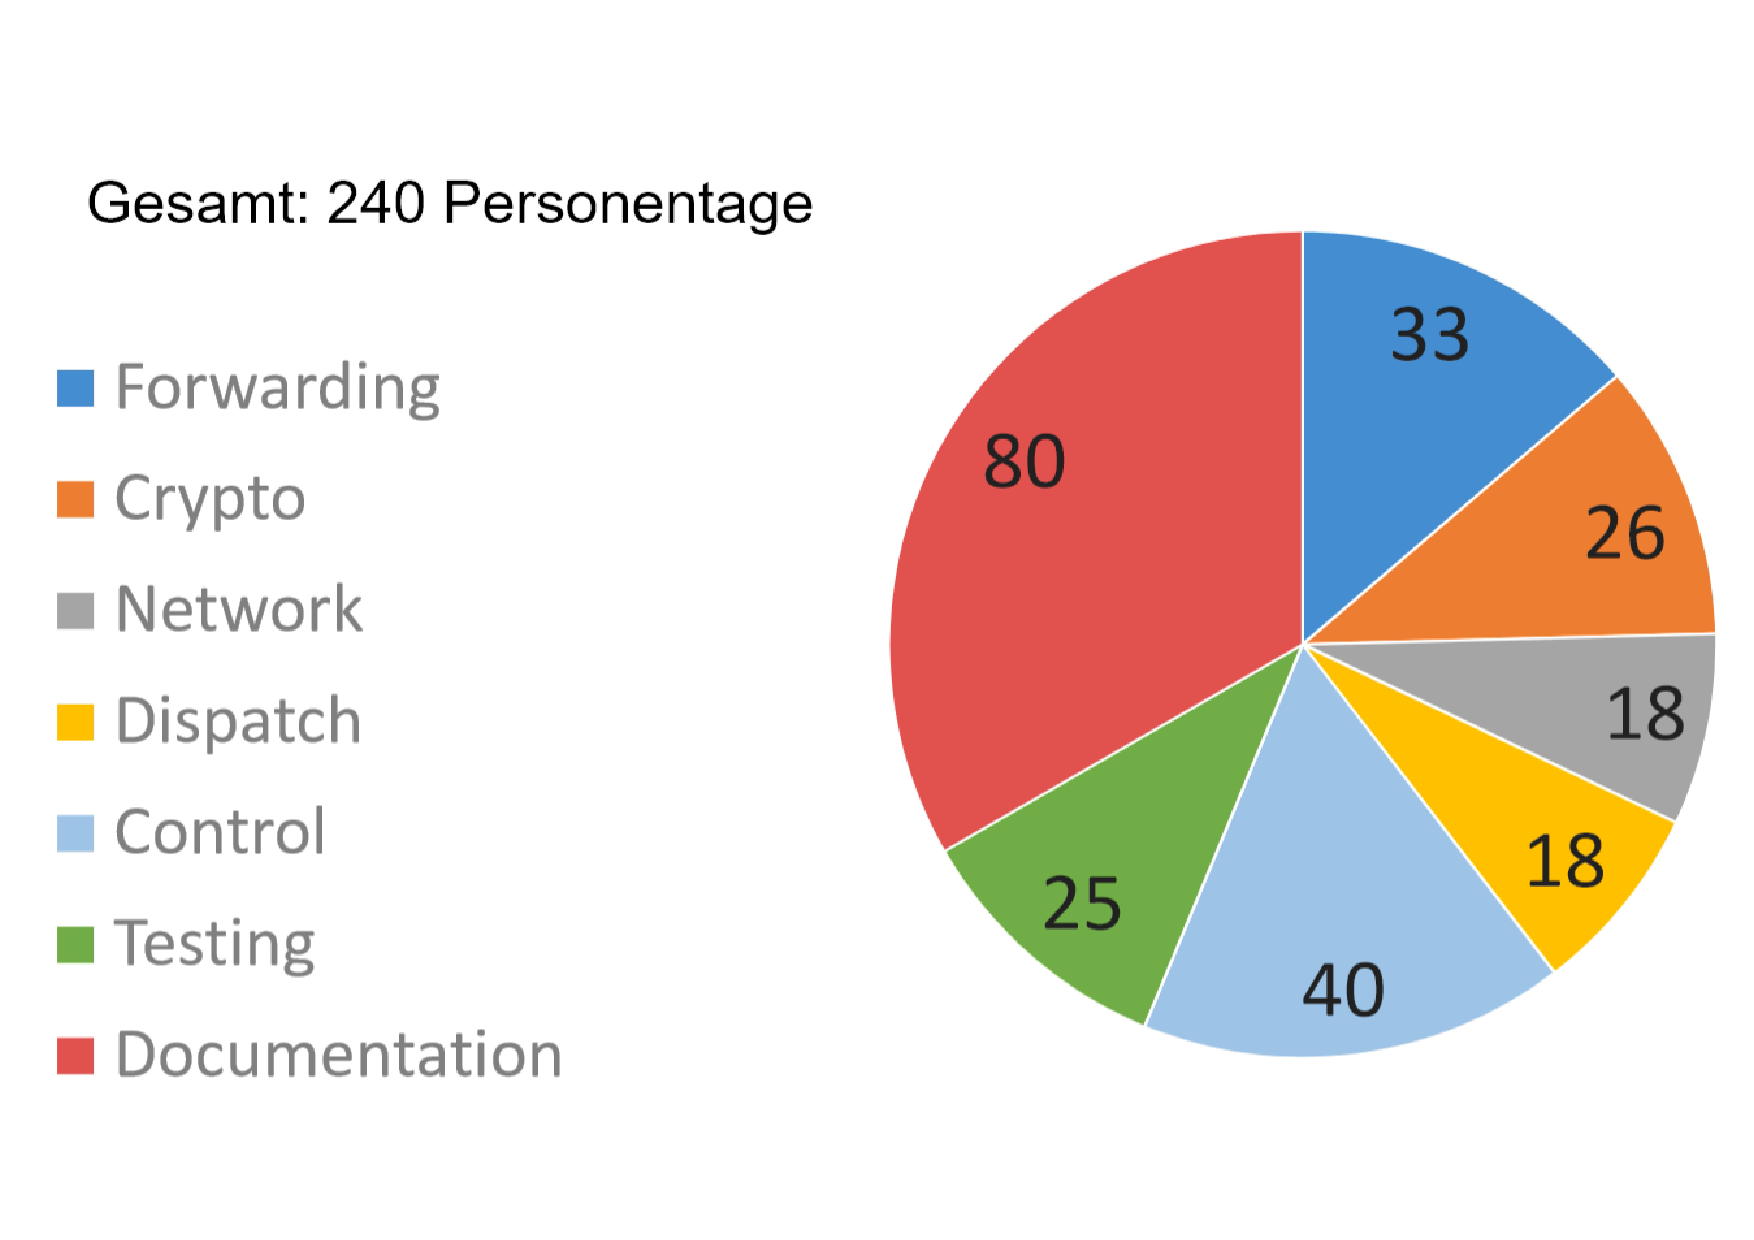
\includegraphics[width= 10cm]{figures/Aufwandsabschaetzung.pdf}
			\caption{Aufwandsabschätzung}
		\end{center}
	\end{figure}

\subsection{Risikoabschätzung}
Bei der Risikoabschätzung wird versucht eine Vorhersage zu treffen, mit welcher Wahrscheinlichkeit bestimmte Risiken eintreffen können und wenn diese eintreffen, welchen Schaden sie im Projekt verursachen. (siehe Abbildung 2)

\begin{figure}
\begin{center}
	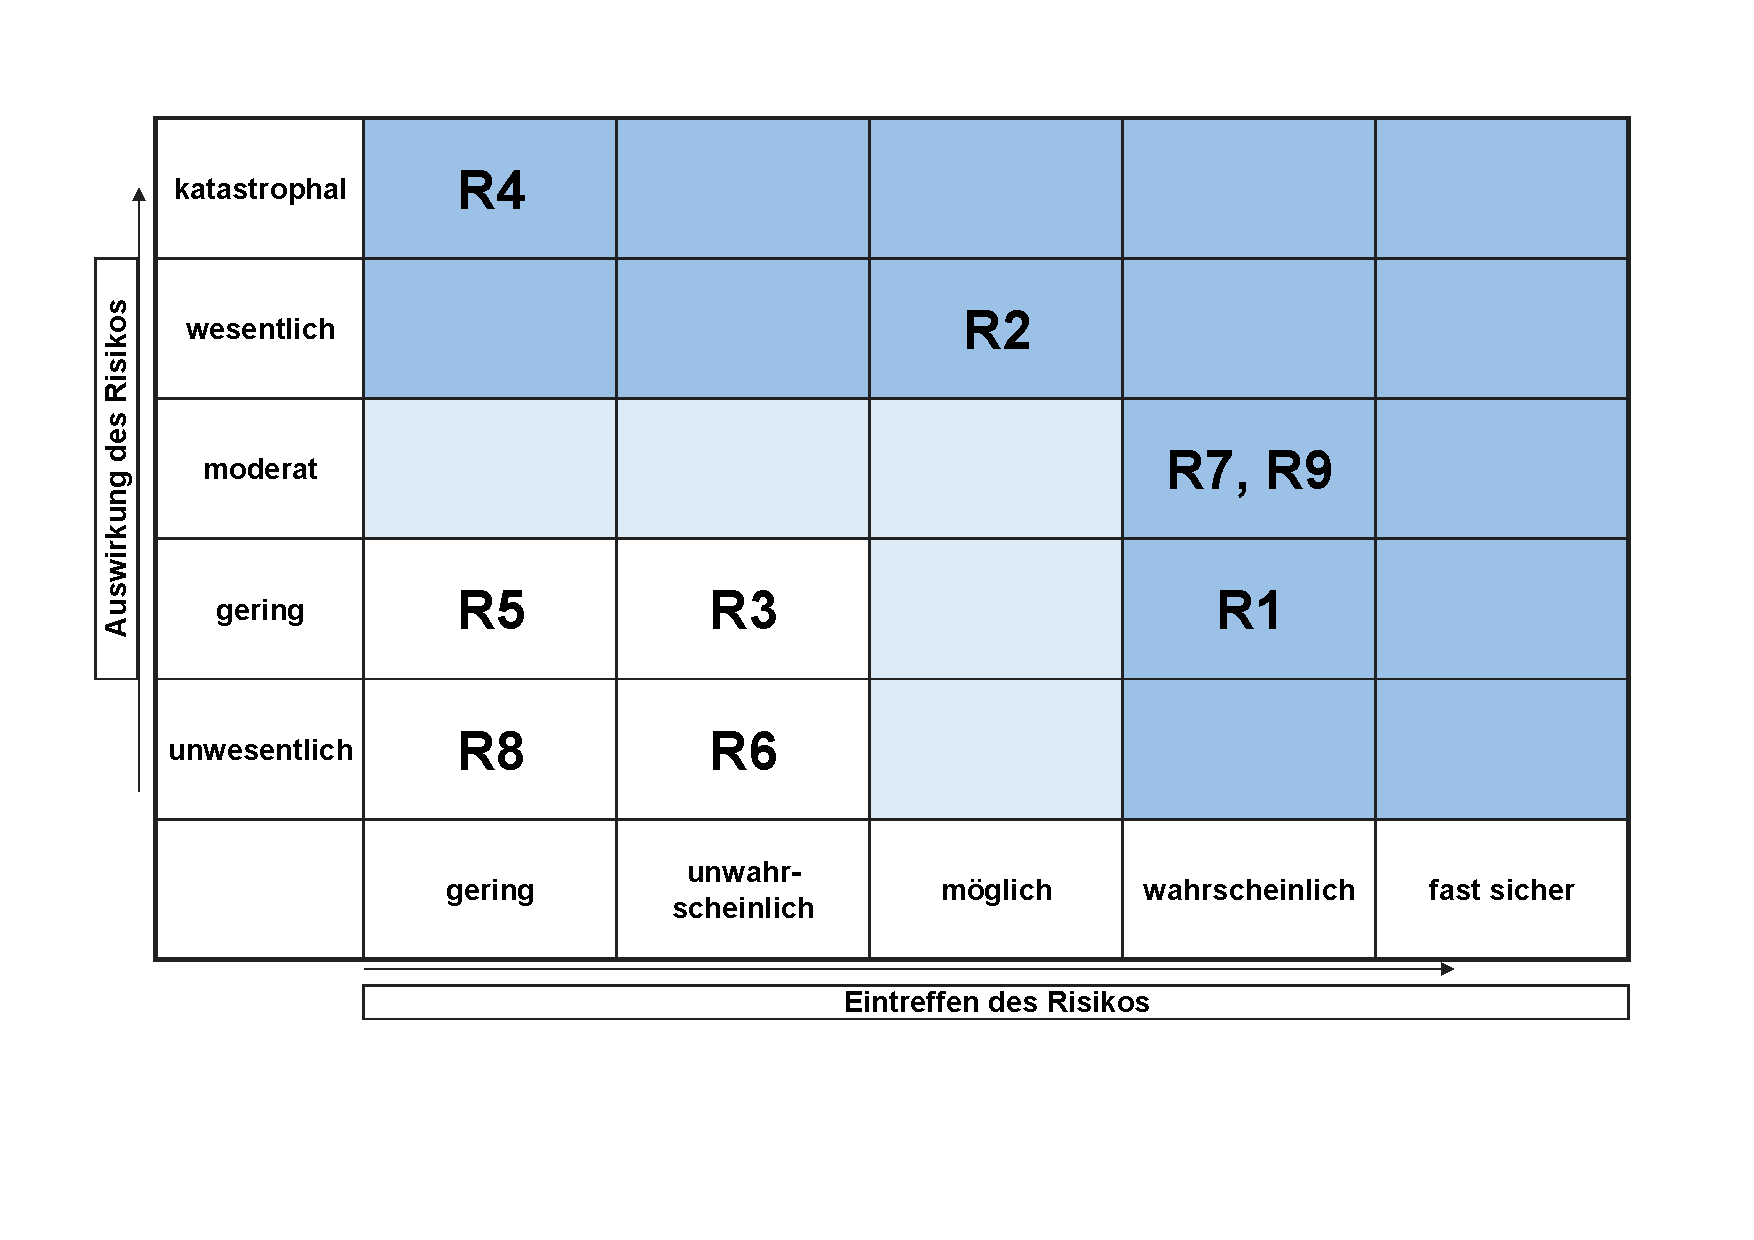
\includegraphics[width= 17cm]{figures/Risikoabschaetzung.pdf}
	\caption{Risikoabschätzung}
	\end{center}
	\end{figure}
	

\begin{description}
		\item[R1:] Kommunikationsprobleme im Team
		\item[R2:] Umfang zu groß
		\item[R3:] Technologie(Rechner) erfüllt nicht die Anforderungen
		\item[R4:] Framework bietet nicht die benötigte Funktionalität
		\item[R5:] Ausfall von Mitgliedern 
		\item[R6:] Anforderungsänderungen durch den Auftraggeber aufgrund eines Kommunikationsproblems im Pflichtenheft
		\item[R7:] falsche Umsetzungsstruktur, gewählte Struktur lässt sich nicht umsetzen
		\item[R8:] Rechtliche Vorgaben
		\item[R9:] versteckte Komplexität
	\end{description}
	
\clearpage
	
\subsection{Meilensteine}
	\begin{description}
	\leftskip=0,8cm
		\item[Erster Meilenstein:] Pflichtenheft, Grobentwurf, lauffähige Implementierung (einfaches Forwarding)
		
		\item[Zweiter Meilenstein:] lauffähige Implementierung (Verschlüsselung mit statischem Schlüssel)
		
		\item[Dritter Meilenstein:] lauffähige Implementierung (Schlüsselaustausch, Gruppenschlüssel), Validierung
	\end{description}
	

	 
\subsection{Organisation}

Die Organisation betrifft alle Regelungen, Vereinbarungen und Aufteilungen der am Projekt beteiligten Personen um ein geordnetes und effizientes Arbeiten zu ermöglichen.
	
\subsubsection{Kommunikationswege}
	\begin{description}
		\item[Zulip:] Dient der schnellen Gruppenkommunikation um effektiv Missverständnisse zu lösen und für eine direkte Kommunikation unter Gruppenmitgliedern.
		
		\item[Email-Verteilerliste:] Dient zur Planung von Treffen und wird für Mitteilungen, die an alle gesendet werden, verwendet.
		
		\item[Gruppentreffen:] Dient zur Diskussion und Besprechung von Problemen. 
		
		\item[Phabricator:] Dient der Zuweisung von Aufgaben an einzelene Gruppenmitglieder und der direkten Kommentierung.
		
	\end{description}
		
\subsubsection{Zusätzliche Vereinbarungen}
	\begin{itemize}
		\item Gruppentreffen jeden Donnerstag von 9:00 Uhr - 12:30 Uhr
		
		\item Kleingruppentreffen nach Absprache und Bedarf
		
	\end{itemize}
		
\subsubsection{Rollenverteilung im Agilen Vorgehen}

	\begin{description}
	\leftskip=0,8cm
		\item[Produkt Owner:] Michael Rossberg
		
		\item[Scrum Master:] Felix Seidel, Tobias Schubert
		
		\item[Entwicklungsteam:] Felix Seidel, Milan Haverkock, Michael Fuchs, Daniel Scheliga, Yannic Faulwetter, Nils Winkelbach, Jörn Weisensee, Tobias Schubert
		
		\item[Kunde, Anwender:] Telematik Lehrstuhl
		
		\item[Management:] Tobias Schubert
	\end{description}

\subsubsection{Organisatorische Rollenverteilung}
	\begin{description}
	\leftskip=0,8cm
		\item[Betreuer:] Michael Rossberg
		
		\item[Teamleiter:] Tobias Schubert
		
		\item[Code:] Felix Seidel
		
		\item[Präsentation:] Daniel Scheliga
		
		\item[Grafik:] Nils Winkelbach
		
		\item[Build-Master:] Milan Haverkock
		
		\item[Dokumentation:] Michael Fuchs
		
		\item[Test:] Jörn Weisensee
		
		\item[Web-Master:] Yannic Faulwetter
		
	\end{description}

\subsubsection{Programmieraufteilung}
	\begin{description}
	\leftskip=0,8cm
		\item[Forwarding]: Milan Haverkock, Daniel Scheliga, Nils Winkelbach
		
		\item[Network]: Felix Seidel, Michael Fuchs, Yannic Faulwetter
		
		\item[Crypto]: Tobias Schubert, Jörn Weisensee
		
		\item[Dispatch]: noch keine genaue Einteilung getroffen
		
		\item[Control]: noch keine genaue Einteilung getroffen
		
		\item[Testing]: noch keine genaue Einteilung getroffen
		
	\end{description}

\clearpage
	
\section{Ergebnisse des Entwurfs}

Die Ergebnisse des Entwurfs sind zum größten Teil in der Entwurfsdokumentation nachzulesen.
Dort sind die Zusammenhänge der verschiedenen Pakete, Komponenten und Klassen aufgezeigt und anschaulich mit Hilfe von UML-Diagrammen dargestellt.

\subsection{Werkzeuge} 

Die verwendeten Werkzeuge sind Softwarelösungen, die die einzelnen Bereiche der Organisation und Entwicklung ermöglichen bzw. erleichtern.

\subsubsection{Organisatorische Werkzeuge}
	\begin{description}
		\item[Phabrikator:] Zuweisung einzelner, zu bearbeitender Tasks und deren Verwaltung, sowie die Bereitstellung des Wiki's. 
		
		\item[Quellcodeverwaltung:]	Hierfür wird \textit{Subversion} benutzt um einen einheitliche Arbeitsgrundlage an den Dateien zu gewährleisten.
		
		\item[Arbeitszeitenerfassung:] Hierfür wird \textit{Kimai} verwendet, dort werden alle Zeiten eingetragen und verschiedenen Themen/Bereichen zugeteilt.
		
		\item[LaTeX:] Hierbei handelt es sich um eine Textbeschreibungssprache, mit der verschiedenste Dokumente erstellt werden können. 
		Diese stehen nach der Erstellung in verschiedenen Formaten zur Verfügung.
		Im speziellen wird es in diesem Projekt für die Erstellung des Pflichtenheftes, den Reviewdokumenten und dem Entwurfsdokument verwendet.   
		
		\item[Doxygen:] Mit diesem Programm werden die Kommentare aus dem erstellten Code gezogen, um daraus eine Dokumentation der Implementierung zu erzeugen.
		
		\item[PlantUML:] Erzeugung von UML-Diagrammen, die Aktivitäten, Aufbau und Funktionen des Systems grafisch darstellen. 
	\end{description}

\subsubsection{Entwicklungswerkzeuge}
	\begin{description}
		\item[Buildsystem:] Es wird \textit{scons} verwendet um eine einheitliche und angepasste Kompilierung von C++-Dateien zu gewährleisten. 
		Hierbei werden sogenannte \textit{sconstruct} erstellt, mit denen verschiedene Vorbedingungen, wie das Einbinden von Bibliotheken und die Auswahl des Kompilers erfüllt werden können.
		
		\item[Entwicklungsumgebung:] Ein beliebiger \textit{Texteditor}, der Syntaxhighlighting für die Programmiersprache C++ unterstützt, wird zum Verfassen des Codes verwendet.
		
		\item[Programmiersprache:] Es wird die hardwarenahe Programmiersprache \textit{C++} verwendet, da diese alle, für das Projekt erforderlichen, Anforderungen erfüllt.
		
		\item[Betriebssystem:] Für den Betrieb der Software ist \textit{Linux} unabdingbar, da das verwendete DPDK-Framework nur auf dessen Grundlage funktioniert.
		
		\item[Bibliotheken:] In diesem Projekt werden viele verschiedene Standardbibliotheken von C++ und vom Auftraggeber bereitgestellte Bibliotheken verwendet. 
		Zusätzlich hierzu wird als spezielles Framework (Ansammlung von Bibliotheken) das DPDK genutzt. 
		Dieses liefert mit seiner umfangreichen Klassensammlung die Grundlage (Verschlüsselung, Forwarding, ...) für das System. 
		
	\end{description}

\subsection{Ergebnisse des Entwurfs für die erste Iteration:}
Die Ergebnisse der ersten Iteration ergeben sich aus dem aktuell zu erreichenden Meilenstein.

\begin{description}
	\leftskip=0,8cm
		\item[Pflichtenheft:] Das Lastenheft wurde vollständig in das Pflichtenheft überführt und um weitere Punkte, im Dialog mit dem Auftraggeber, ergänzt.
		
		\item[Grobentwurf:] Der Grobentwurf umfasst eine erste Übersicht über die Funktions- und Arbeitsweise des Systems.
		
		\item[Implementierung:] Eine erste Lauffähige Implementierung wurde umgesetzt und umfasst die Funktionen eines einfachen Forwardings ohne Verschlüsselung.
		
		\item[Planung:] Es wurden Festlegungen für die weiteren Iterationen getroffen, hierbei wurden insbesondere die Meilensteine für die nächste Iteration festgelegt und das weitere Vorgehen innerhalb des Teams besprochen.
		
	\end{description}

\subsection{Festlegungen für die nächste Iteration:}
Die Festlegungen für die jeweilige nächste Iteration spiegeln sich in den Meilensteinen wieder.

\begin{description}
	\leftskip=0,8cm
		\item[Grobentwurf verfeinern:] Der Grobentwurf wird um spezifischere Diagramme und Beschreibungen zum Feinentwurf ergänzt. Dies geschieht jeweils parallel zu den Meilensteinen, da automatisch jede Änderung dort festgehalten wird.
		
		\item[Implementierung erweitern:] Die aktuelle Implementierung wird um einen ersten Entwurf der Verschlüsselung mit statischem Schlüssel erweitert.
		
		\item[Hardware konfigurieren:] Die zur Verfügung gestellte Hardware wird initial konfiguriert um die Voraussetzungen für das System zu gewährleisten und um die Implementierung ersten Tests unterziehen zu können.
		
	\end{description}
  
\end{document}
